% !TeX spellcheck = hu_HU
% !TeX encoding = UTF-8

%----------------------------------------------------------------------------
\chapter{Gyakorlati eredmények}
%----------------------------------------------------------------------------
Ebben a fejezetben alkalmazom a korábbiakban megismert elméleti módszereket, megvizsgálom milyen futásidőt érnek el különböző megoldóprogramok használatával.
%, illetve összevetem az így kapott eredményeket a kombinatorikus algoritmusok hatékonyságával.

Az implementációkat a Google által üzemeltetett Colaboratory segítségével készítettem Python nyelven. A választás többek között azért esett erre a rendszerre, mert a D-Wave Systems által, Python nyelven publikált könyvtárat szerettem volna felhasználni, és ez így nem csak minimális konfigurációval megoldható, de az eredmények könnyen rekonstruálhatók a konténer technológia miatt, és nem befolyásolják őket a lokális, saját gépen eszközölt módosítások.

A teszteléshez generált gráfok előállításához és reprezentálásához a NetworkX könyvtárat használtam fel \cite{NetworkX}.

\section{QUBO-k megoldása}

A D-Wave Ocean nevű programcsomagja több lehetőséget kínál QUBO formák megoldására. Van egzakt megoldója, ez azonban nagyon kicsi bemenetekre is használhatatlan a gyakorlatban, hiszen működési elvét tekintve, minden lehetőséget kipróbál. Ezen kívül van lehetőség kvantum számítás szimulálására, vagy egy valós kvantumgépnek is elküldhetjük a problémát a megfelelő API használatával \cite{DWaveOcean}.

Lényeges észrevétel, hogy a D-Wave megoldója - az energiaminimumra törekvés elve alapján - csak minimalizálni tud, ezért a korábban bemutatott QUBO-kat is ilyen alakra kell hozni. Ez szerencsére könnyen megy, mert ha eredetileg maximalizálni szerettünk volna, egyszerűen minden tagot $-1$-gyel kell megszoroznunk, és az így kapott függvényt minimalizálni.

A helyes konfiguráció után van lehetőségünk a korábban bemutatott QUBO modellek tényleges próbájára.

A szimulált kvantumgépen való megoldás mellett két fő iránya van a D-Wave számítógépek használatának. Ebből az egyik a direkt módon beágyazása a problémának kvantumszámítógépre, a mások pedig egy hibrid megoldót használ, mely klasszikus optimalizációkat is végez.

A direkt QPU-t (Quantum processing unit) használatával sajnos probléma ütköztünk, ahogy nőtt a probléma mérete, nem túl nagy, vagyis pár száz csúcsot tartalmazó gráfokra is túl hosszú volt a beágyazás, és időnként túl sokat kellett kvantum erőforrásra is várni. Sajnos nem is teljesen sikerült kideríteni, hogy ennek miért van köze a probléma méretéhez, de nagyobb bemenetek esetén jellemzőbb volt ez a viselkedés. Azért is érdekes, mert a probléma megoldása a QPU-n hamar elkészül (amennyiben eljut odáig), amely kiderül a jelentésekből. Az erőforrásra várakozás azért tűnik valószínűnek, mert a kliens, ahonnan a hívást végzem többször egy \verb+get_solvers+ nevű függvény belsejében várakozik. Ugyanakkor viszont nem ez tűnik az egyetlen oknak, hiszen kisebb problémák megoldásánál nem jelentkezik ez a probléma, így azt is sejtjük, hogy a probléma beágyazása valamiért nem történik meg hatékonyan.\\

A D-Wave rendszer esetén a QUBO megadására a Python collections könyvtárának defaultdict osztályát használom, ahol kulcsként adom meg a változópárt, amelyen a kapcsolatban állnak, értékként pedig a szorzatukhoz tartozó együtthatót. Mivel elsődlegesen a D-Wave-et használom, mint megoldószoftvert, így a példakódokban is így konstruálom meg a QUBO-t, azaz, egy Q defaultdict osztályt használok.


A QUBO-kat, és általánosságban a kvadratikus programozási feladatokat persze más, klasszikus megoldóprogramokkal is megoldathatjuk. A D-Wave maga is publikál egy qbsolv nevű csomagot, melyen kvantum erőforrások használata nélkül is lehetőség van a QUBO megoldására. A dokumentáció szerint ez képes megtalálni nagy QUBO problémák optimumát, a probléma részproblémákká bontásával, miközben egy klasszikus megoldót használ, amely a tabu algoritmust futtatja \cite{DWaveOceanQbsolv}. 

Egy kereskedelmi forgalomban lévő, egyik piacvezető lineáris programozás megoldó szoftver a Gurobi, melynek bár nem fő iránya a kvadratikus programok megoldása, ezeket is támogatja \cite{gurobi}. 

Sajnos az eredmények viszont itt sem voltak biztatóak, viszonylag kevés változószámnál is reménytelennek tűnt egy általános QUBO megoldása, illetve nem sokkal később az ingyenes licenc korlátaiba ütköztünk, amennyiben túl sok változót szerettünk volna hozzáadni a modellhez. Az akadémia licenc igénylése kutatási célokra ugyan egyszerűen működik, ezek a licencek nem kompatibilisek konténerizált környezetekel, így a Colaboratory-ban sem használhatók. Egy viszonylag új licencelési módszer a Web License Service (WLS) használata, azonban bár a konfiguráció egyszerű, megfelelő dokumentáció hiányában, napok munkája volt ezt megfelelően elvégezni.

Ha mindent jól beállítottunk, akkor például a korábban elkészített Q szótárat is átkonvertálhatjuk Gurobi modellé, és megoldhatjuk a problémát, így kapva egy QUBO megoldót. Persze, érdemes észben tartani, hogy a Gurobi nem fő profilja a kvadratikus optimalizálás, és ha lehet, akkor érdemes korlátként hozzávenni a kényszereket, ahelyett, hogy azokat a büntetőtagokként a célfüggvénybe fogalmaznánk bele. Alább látható egy példakód, amellyel a már felépített QUBO-t tudjuk megoldani, végeredményként ugyanolyan típúsú look-up-table (lut)-t kapva, amelyet a D-Wawe válaszából is ki tudunk nyerni. Azaz a lut i. eleme megmondja, hogy az i. változó értéke 0 vagy 1.


\begin{lstlisting}[language=python,caption=Max-cut QUBO,label=code:solveQUBOWithGurobi]	
def solveQUBOWithGurobi(Q):
	model = gp.Model('ModelFromQUBO', env=gurobiEnv)
	X = defaultdict(lambda: model.addVar(vtype=GRB.BINARY))
	expr = gp.QuadExpr()
	for ((u, v), w) in Q.items():
		expr.add(w*(X[u]*X[v]))
	
	model.setObjective(expr, GRB.MINIMIZE)
	
	model.optimize()
	
	lut = dict()
	for var in sorted(X):
		lut[var]=X[var].X
	
	return lut
	
\end{lstlisting}


\section{Gráf generálása}
Az alkalmazások ellenőrzésére speciális gráfokat generáltam, melyen így előre meg tudtam határozni a várható minimális, illetve maximális vágásokat.
A generált gráf rendelkezik négy különböző paraméterrel, ezek $N$, $K$, $p$ és $q$.
A gráfot ezek után jelöljük $G(N,K,p,q)$-val.
Az ötlet csupán annyi, hogy előre meghatározunk $K$ darab diszjunkt halmazt, hogy mindegyik csoportban pontosan $N$ darab csúcs legyen. Ezután minden élről egyénileg döntünk, hogy őt hozzávesszük-e a gráfhoz. Amennyiben egy él egy csúcs $N$-esen belül fut, ez a valószínűség legyen $q$, amennyiben két különböző csúcs $N$-es között fut, akkor legyen ez a valószínűség $p$. Világos, hogy ha $p$ kicsi, $q$ pedig nagy, akkor $K$ klasztert kapunk, ahol az élek sűrűek, a csoportok között viszont ritkák. Ellenkező esetben $K$ darab egymástól majdnem független ponthalmazt kapunk, ahol a halmazok között viszont sok él hozzá van adva a gráfhoz. Az előbbivel egy minimális vágás várhatóan a $K$ klasztert szétválasztó vágás lesz, utóbbi esetben pedig ugyanígy a maximális vágásra lesz egy jó becslésünk.

Érdemes megvizsgálni az elfajuló eseteket. $G(N,K,0,1)$ esetén $K$ darab különálló egyenként $N$ csúcs teljes gráfot kapunk. $G(N,K,1,0)$ esetén pedig ennek a komplementerét kapjuk. 

Az élsúlyokat pedig egy véletlenszámmal generáltam minden élre, a példákban mindenhol 0 és 1 közötti egyenletes eloszlással, holott ez a példakódban paraméter segítségével állíthatóan oldottam meg.

Érdemes észben tartani, hogy $n=|V|=N \cdot K$, tehát a kicsi $n$ és nagy $N$ nem keverendő.

TODO: Néhány példakód

%%----------------------------------------------------------------------------
%\section{Minimális vágás}
%%----------------------------------------------------------------------------
%
%
%\subsection{Klasszikus}
%
%A probléma klasszikusan is megoldható, például folyamalgoritmus segítségével. Referenciaként a NetworkX-ben ilyen módon implementált \verb+minimum_cut+ függvényt fogom használni.
%
%\begin{lstlisting}[language=Python,caption=Min-cut flow,label=code:minCutFlow]
%	cut_value, partition = nx.minimum_cut(G, s, t, 'weight')
%\end{lstlisting}
%
%
%\subsection{QUBO}
%Egy $n$ változós bináris kvadratikus kifejezést megadhatunk tömören mátrixos formában is, ahol a $Q$ mátrix $q_{ij}$ eleme az $x_i x_j$ együtthatója. Mivel ezt a formát képes kezelni a legtöbb a megoldó, (vagy ha nem, akkor könnyen átalakítható olyan formára) ezért a továbbiakban ilyen formában adjuk meg.
%
%A minimális vágás problémája könnyen felírható QUBO-ként, ahogyan azt korábban is láttuk. Az egyetlen "trükk", hogy két speciális pontot ki kell jelölni, amelyeknek külön csoportba kell kerülniük. Mivel azonban ez a klasszikus folyamalgoritmusnál is így működik, ezért ilyen tekintetben ez a megoldás sem alsóbbrendűbb.
%
%\begin{lstlisting}[language=python,caption=Min-cut QUBO,label=code:minCutQUBO]
%	for u, v in G.edges:
%		w=G.edges[u,v]['weight']
%		Q[(u,u)]+= 1*w
%		Q[(v,v)]+= 1*w
%		Q[(u,v)]+= -2*w
%	
%	Q[(s,s)]+=inf
%	Q[(t,t)]-=inf
%\end{lstlisting}

%----------------------------------------------------------------------------
\section{Maximális vágás}
%----------------------------------------------------------------------------

A maximális vágás klasszikus példája a QUBO-nak, ezt könnyen elintézhetjük.
%Éppen úgy működik, mint a minimális vágás, de nem szükségesek a büntető tagok.
Érdemes megfigyelni, hogy a változók száma pontosan $|V|=n$.

\begin{lstlisting}[language=python,caption=Max-cut QUBO,label=code:maxCutQUBO]
	for u, v in G.edges:
		w=G.edges[u,v]['weight']
		Q[(u,u)]+= -1*w
		Q[(v,v)]+= -1*w
		Q[(u,v)]+= 2*w
\end{lstlisting}


Az egyszerű maximális vágásra felírt QUBO-t szinte minden megoldó szoftver jól kezelte. Nagy bemenetekre is általában pontos eredményt kaptunk vissza. A leglassabb megoldónak a Gurobi bizonyult, de a képet árnyalja, hogy az ő szoftverük pontosan megkeresi az optimum értékét. Így bár viszonylag hamar megtalál egy optimumhoz nagyon közeli értéket, vagy akár magát az optimumot, a primál feladatból készített duális megoldása sokáig tart neki. Így érdemes lehet befolyásolni a megoldót, hogy ne pontos megoldást keressen, hanem megengedjük egy bizonyos hibaszázalékot.

A TODO táblázat, illetve \refstruc{fig:maxCutQUBO} foglalja össze a különböző módszerekkel kapott futásidőket.

\begin{figure}[!ht]
	\centering
	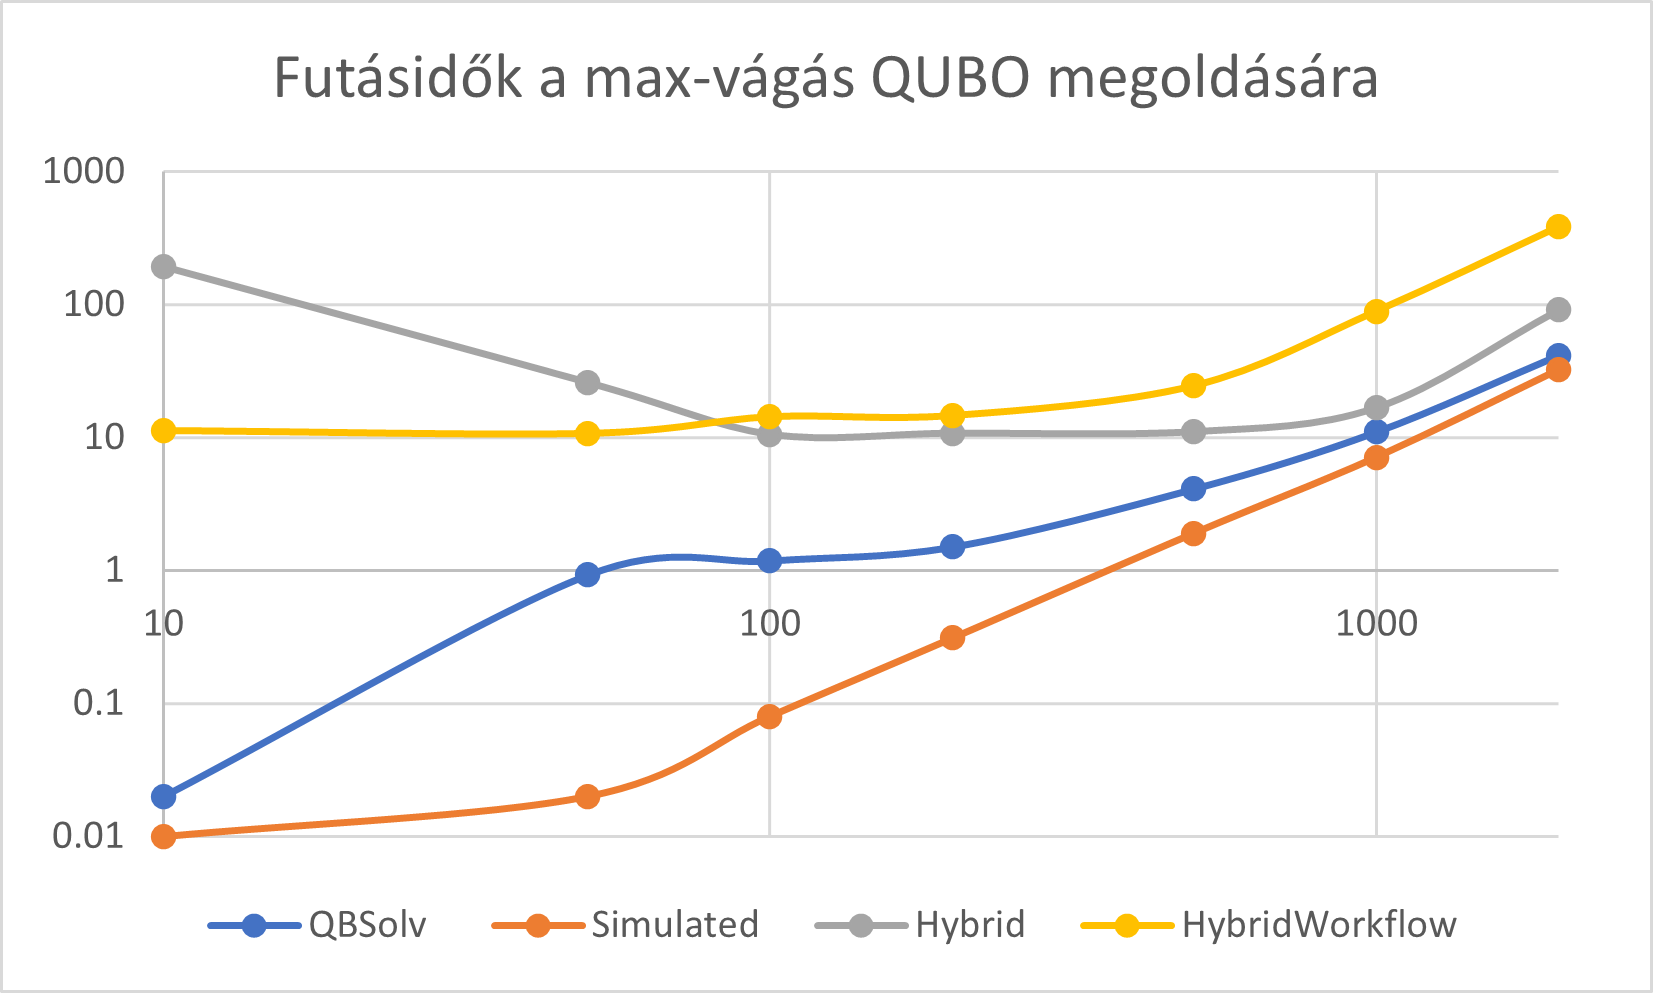
\includegraphics[width=150mm, keepaspectratio]{figures/diagrams/maxCutQUBO.png}
	\caption{Futásidők a max-vágás QUBO megoldására}
	\label{fig:maxCutQUBO}
\end{figure}

TODO: a grafikont még alakítom + eredmények elemzése
Hasonló grafikonokat képzelek a max-vágás témaköréhez is.

A diagramcím mindkét helyen szerepeljen?

%----------------------------------------------------------------------------
\section{Maximális K-vágás (one-hot encoded)}
%----------------------------------------------------------------------------

A maximális K-vágásnál több trükköt is be kellett vetnünk. Az elméleti megfontolásokon felül, itt már csupán annyit kell még kezelni, hogy a változókat jól osszuk ki. Vagyis amíg az $x_{ui}$ változót kettő indexszel indexeltük, az elméleti felírásban, most egy indexszel kell megadnunk egyértelműen, hogy a mátrixos formába leképezhető legyen.
\footnote{Igazából ez nem szükségszerű, mert a mátrix felírásához, a Python dict típusa miatt, akár sztringeket is használhatunk kulcsként, vagyis a sor-oszlop koordináták azonosítására. Ezt a következő példában ki is használom, de ennél a feladatnál még könnyen kezelhetőek az indexek leképezése is.}
Ezt pedig úgy oldjuk meg, hogy a változókat sorba rakva blokkonként következnek az egy csúcshoz tartozó változók, azaz $x_{ui}$ az $(uK+i)$. változó lesz. Ennek megfelelően használjuk tehát az indexeket.

Ebből következik továbbá az a korábbi, de fontos megfigyelés is, hogy a változók száma itt $n \cdot K = N \cdot K^2$.

\begin{lstlisting}[language=python,caption=Max-K-cut QUBO (szimmetrikus mátrix), label=code:maxKCutQUBOSymmetric]
for u, v in G.edges:
	for i in range(K):
		for j in range(K):
			if (i!=j):
				w=G.edges[u,v]['weight']
				Q[(u*K+i,v*K+j)] += -1*w

for u in range(K*N):
	for i in range(K):
		for j in range(K):
			if (i!=j):
				Q[(u*K+i,u*K+j)] += inf 
\end{lstlisting}

\begin{lstlisting}[language=python,caption=Max-K-cut QUBO (háromszög mátrix),label=code:maxKCutQUBOTriangle]
for u, v in G.edges:
	for i in range(K):
		for j in range(i+1, K):
			w=G.edges[u,v]['weight']
			Q[(u*K+i,v*K+j)] += -1*w
			Q[(v*K+i,u*K+j)] += -1*w

for u in range(K*N):
	for i in range(K):
		for j in range(i+1, K):
			Q[(u*K+i,u*K+j)] += inf
\end{lstlisting}

Mivel úgy éreztem, hogy a korlátok célfüggvénybe való beleerőltetése nem előnyös akkor, ha a megoldóprogram amúgy támogatja korlátok megadását is, így a Gurobi-t nem csak a nyers QUBO megoldására használtam, hanem felhasználtam a korlátokat külön hozzáadva, és csak a ténylegesen optimalizálandó részeket célfüggvényként megadva. Ezzel várhatóan jobban teljesítsen... TODO


TODO: az alábbi szöveget és táblázatot 
frissíteni az új mérésekre vonatkozólag:

A maximális K-vágásra pár futásidőt szemléltetően, egy táblázatot készítettem néhány gráfra. A táblázat első két sorában a $K=2$ eset miatt, az egyszerű maximális vágásnál látott módon oldottam meg, amíg a 3-4. sorban az általános K-vágást alkalmaztam ugyanarra a gráfra. A gráfoknál $p=0.9$ és $q=0.1$ paramétereket használtam, így ezeket nem jelöltem külön.

A futásidőknél sokszor jellemzőek voltak akár 1-2 másodperces eltérések is ugyanarra a bemenetre, a sok külső befolyásoló tényező miatt. (Kezdve csak azzal, hogy a Hibrid esetnél interneten keresztüli kommunikációval oldjuk meg a problémát, ezért csak a hálózati kommunikáció egy elég jelentős állandón változó tényező.) Mindezért csak közelítőleg másodperces pontosságot használtam.

A vágások várható optimumát is feltüntettem  ezresekre kerekítve. Ez egyrészt kijön a saját méréseimből, másrészről, ha $p=1, q=0$ közelítést használjuk, akkor $N \approx (N-1)$ miatt, expliciten kiszámolható a $\binom{K}{2} \cdot N^2 \cdot E(W)$, képlettel, ahol $E(W)$ az élsúlyok várható értéke.

$inf$ értékére egységes mindenhol $10000$ használtam.

\begin{table}[ht]
	\footnotesize
	\centering
	\begin{tabular}{ l c c c }
		\toprule
		Gráf & Vágás optimuma & Szimulált kvantum (s) & Hibrid (s) \\
		\midrule
		$G(N=100, K=2, p, q)$ & $5000$ & 0.37 & 2.5   \\
		$G(N=1000, K=2, p, q)$ & $500000$ & 32.5 & 11.5 \\
		$G(N=100, K=2, p, q)$ & $5000$ & 0.9 & 3.5  \\
		$G(N=1000, K=2, p, q)$ & $500000$ & 73 & 21 \\	
		$G(N=100, K=3, p, q)$ & $15000$ & 6 & 2.5 \\		
		$G(N=50, K=4, p, q)$ & $7500$ & 6 & 3 \\		
		$G(N=100, K=4, p, q)$ & $30000$ & 25 & 8 \\

		\bottomrule
	\end{tabular}
	\caption{Futásidők különböző gráfokra}
	\label{tab:TabularExample}
\end{table}

Sajnos a futási idők elemzése önmagában nem elég, fontos megvizsgálni, hogy valóban jó (közelítő) eredményeket kaptunk-e. $K=2$ esetre minden esetben megtaláltuk az optimumot, bármely elkódolást is használjuk.
Sajnos $K>2$ esetre viszont elképesztően rossz vágásokat kaptunk vissza. Például az utolsó esetben a 30000 körüli vágásérték helyett a szimulált kvantum esetén 23000 körüli értéket kaptunk. Amely nem csak, hogy az optimumtól nagyon távol esik, (több mint $20\%$), hanem ha végig gondoljuk, egy véletlenszerű vágás, amikor a $K$ csoport mindegyikébe minden eredeti csoport $K$-ad részét tesszük, akkor is várhatón ilyen körüli vágást kell kapjunk. Ugyanis ha $p=1, q=0$, akkor $K \cdot \frac{N}{K} \cdot (N-\frac{N}{K}) \cdot \binom{K}{2}$ adja az élek számát, amelyet még szorozni kell az élsúlyozás várható értékével. Ez az utolsó példára $22500$-at ad. A kapott felosztáson továbbá "szemmel végignézve" is úgy tűnik, mintha véletlen felosztásról lenne szó.
Hibrid számításnál általában valamivel jobb a eredményeket kapunk, és a felosztás megvizsgálásánál is olykor látszik, hogy a csúcsok mintha lassan elkezdenének megfelelően csoportokba tömörülni, azonban még mindig alig kapunk jobbat egy véletlenszerű vágásnál.

Azt sejtjük hogy valamilyen paraméterek konfigurálásával javítható lenne ez az eredmény, de egyelőre, a viszonylag kicsi felhasználóbázis és elérhető dokumentáció miatt nem sikerült ezt kideríteni. Az is elképzelhető, hogy az általam adott elkódolásban van a hiba, viszont ekkor érdekes, hogy $K=2$ esetre mindkét módszer hibátlanul működik.  Az viszont sajnos kiderült, hogy ebben a formájában a megoldó nem alkalmazható, hiszen mint láttuk, viszonylag kicsi (néhány száz csúcsból álló) gráfokra sem ad még jó közelítést sem.

%----------------------------------------------------------------------------
\section{Maximális K-vágás (binary encoded)}
%----------------------------------------------------------------------------

Mivel a korábban bemutatott elmélet alapján rengeteg segédváltozó bejön, így nehéz lett volna a természetes számok halmazára leképezni az összes változót, és így felírni a mátrixot. Ezért a QUBO definiálásánál kihasználtam, hogy a defaultdict kulcsainak nemcsak egész számokat, hanem akár stringeket (pontosabban string párokat) is megadhatunk, így string-ként kezelve a változóneveket kicsit követhetőbb a folyamat. Ezáltal a kódban a csoportokat elkódoló változókat \verb+x_u_i+-vel jelöltem, melynek jelentése továbbra is, az $u$ csúcs csoportját elkódoló szám i. bitje. \verb+d_u_v_i+-vel jelöltem, hogy az $u$ és $v$ csoportját elkódoló számok i. bitje különbözik-e, illetve \verb+dtemp_u_v_i+-vel a XOR kapu használatánál szükséges segédváltozót. Ennek mintájára \verb+D_u_v+ jelöli az $u$ és $v$ különböző csoportba kerülését. Ezen kívül további változók jönnek majd be az \verb+or_gate_list+ meghívásánál, ott a függvényen belül adom hozzá a Q-hoz az új változókat, úgy hogy azok nevükben egyediek legyenek, méghozzá a kimeneti változónév mögé mindig hozzákonkatenálom, hogy a lista mely indexű elemeit állítja OR kapcsolatba.

A kód egyébként két nagyobb részből áll, egyrészt a \verb+D_u_v+ változók előállítása, másrészt a  \verb+D_u_v+ változókat össze kell szorozni a megfelelő súlyokkal.

\begin{lstlisting}[language=python,caption=Max-K-cut QUBO (bináris kódolás),label=code:maxKCutQUBOBinary]

import math

# Initialize our Q matrix
Q = defaultdict(int)

# k is the number of bits needed to write a groupnumber
k = math.ceil(math.log2(K))

# Define the D_u_v variables with constraints
for u in range(K*N):
	for v in range(u+1, K*N):
		x_ui="x_"+str(u)+"_"+str(i)
		x_vi="x_"+str(v)+"_"+str(i)
		d_uvi="d_"+str(u)+"_"+str(v)+"_"+str(i)
		dtemp_uvi="dtemp_"+str(u)+"_"+str(v)+"_"+str(i)
		xor_gate(Q,x_ui,x_vi,d_uvi,dtemp_uvi)
		listOfds.append(d_uvi)
		or_gate_list(Q, listOfds, "D_"+str(u)+"_"+str(v))

# Update Q matrix for every edge in the graph
for u, v in G.edges:
	w=G.edges[u,v]['weight']
	Q[("D_"+str(u)+"_"+str(v),"D_"+str(u)+"_"+str(v))] += -1*w

\end{lstlisting}

\subsection{Logikai kapuk megvalósítása}

A fenti módszer működéséhez azonban implementálni kell a logikai kapukat is.
Ezek az elemi kapuk esetében nem okoznak különösebb problémát, hiszen a korábbi fejezetben már megadtuk, hogy milyen együtthatókat kell használni, így az implementálásnál elég egyszerűen paraméterként átvenni egy Q objektumot, melybe a változók együtthatói elmentésre kerülnek, és magukat a változókat azonosító neveket, melyekre a logikai összefüggést alkalmazni akarjuk. A Q mátrix megfelelő mezőihez hozzáadjuk a korábban kiszámolt együtthatókat, és ezzel kész is vagyunk.

\begin{lstlisting}[language=python,caption=Elemi kapuk,label=code:ElementaryGates]
	
def same(Q, in1, in2):
	Q[(in1,in2)] -= 2*p
	Q[(in1,in1)] += 1*p
	Q[(in2,in2)] += 1*p

def and_gate(Q, in1, in2, out):
	Q[(in1,in2)] += 1*p
	Q[(in1,out)] -= 2*p
	Q[(in2,out)] -= 2*p
	Q[(out,out)] += 3*p

def or_gate(Q, in1, in2, out):
	Q[(in1,in2)] += 1*p
	Q[(in1,out)] -= 2*p
	Q[(in2,out)] -= 2*p
	Q[(out,out)] += 1*p
	Q[(in1,in1)] += 1*p
	Q[(in2,in2)] += 1*p

def xor_gate(Q, in1, in2, out1, out2):
	Q[(in1,in2)] += 2*p
	Q[(in1,out1)] -= 2*p
	Q[(in2,out1)] -= 2*p
	Q[(out1,out1)] += 1*p
	Q[(in1,in1)] += 1*p
	Q[(in2,in2)] += 1*p
	Q[(out2,out2)] += 12*p
	Q[(out1,out2)] += 4*p
	Q[(in1,out2)] -= 8*p
	Q[(in2,out2)] -= 8*p
	
\end{lstlisting}

A több-bemenetű OR kapura is készítettem egy rövid függvényt, amely elvégzi az OR műveletet az összes bemenetére. Mindezt úgy teszi, hogy közben felépít egy bináris fát OR kapukból, időközben segédváltozókat bevezetve. Implementációját tekintve "oszd meg és uralkodj" elven működik, vagyis rekurzívan meghívja saját magát a paraméterként átadott tömb első-, illetve második felére, majd a kapott eredményekre alkalmazza az OR műveletet.

\begin{lstlisting}[language=python,caption=Elemi kapuk,label=code:MultipleOrGates]
	
def or_gate_list(Q, in1, out):
	length = len(in1)
	if (length==1):
	same(Q, in1[0], out)
	return
	
	half = length // 2
	out1 = out +"_0-" +str(half)  
	out2 = out +"_" +str(half) + "-" +str(length)
	or_gate_list(Q, in1[:half], out1)
	or_gate_list(Q, in1[half:], out2)
	or_gate(Q, out1, out2, out)
	
\end{lstlisting}

Illetve segédfüggvényként létrehoztam még egy bitenkénti XOR műveletet végző függvényt, mely csak annyit csinál, hogy a bemenetként kapott két listára elempáronként alkalmazza a korábban definiált \verb+xor_gate+ függvényt.

\begin{lstlisting}[language=python,caption=Elemi kapuk,label=code:XorGateList]
	
def xor_list(Q, in1, in2, out1, out2):
	for i in range(len(in1)):
		xor(Q, in1[i], in2[i], out1[i], out2[i])
	
\end{lstlisting}

\subsection{Maximális-K-vágások összehasonlítása}

